% =====================================================================
%  KARIOS CubeSat -- SysML System Model : rendered diagram views
%  Companion to KARIOS_system_model.sysml
%
%  Views: bdd (Structure) | req (Requirements) | uc (Use Cases)
%         stm (State Machine) | par (Parametrics)
%
%  Compile:  pdflatex KARIOS_sysml_diagrams.tex   (run once)
% =====================================================================
\documentclass[landscape,a4paper,10pt]{article}
\usepackage[T1]{fontenc}
\usepackage[margin=12mm]{geometry}
\usepackage{helvet}
\renewcommand{\familydefault}{\sfdefault}
\usepackage{tikz}
\usetikzlibrary{positioning,arrows.meta,fit,backgrounds,calc,shapes.multipart,shapes.geometric}
\pagestyle{empty}

\definecolor{accent}{HTML}{2563A8}
\definecolor{ink}{HTML}{131B28}
\definecolor{ink3}{HTML}{6B7788}
\definecolor{line}{HTML}{C4CDD9}
\definecolor{surface}{HTML}{FFFFFF}
\definecolor{surface2}{HTML}{EEF3F9}
\definecolor{creq}{HTML}{2F74C0}
\definecolor{cstr}{HTML}{1F8F86}
\definecolor{cbeh}{HTML}{7C53A5}
\definecolor{cpar}{HTML}{C9761F}

% ---- common styles ----
\tikzset{
  blk/.style={draw=ink, line width=0.6pt, rectangle split, rectangle split parts=2,
              fill=surface, align=center, inner sep=3pt, font=\scriptsize, text width=2.5cm},
  blk1/.style={draw=ink, line width=0.6pt, rounded corners=1pt,
               fill=surface, align=center, inner sep=4pt, font=\scriptsize, text width=2.5cm},
  ster/.style={font=\scriptsize\itshape, text=ink3},
  compo/.style={{Diamond[open=false,length=2.8mm,width=2.1mm]}-, line width=0.6pt, draw=ink3},
  assoc/.style={line width=0.5pt, draw=ink3},
  satis/.style={-{Triangle[open,length=2.6mm,width=2.6mm]}, dashed, line width=0.6pt, draw=creq},
  uc/.style={draw=cbeh, line width=0.7pt, ellipse, fill=surface, align=center,
             font=\scriptsize, inner sep=1pt, minimum width=3cm, minimum height=1.15cm},
  actor/.style={draw=ink, line width=0.6pt, rounded corners=1pt, fill=surface2,
                align=center, font=\scriptsize, inner sep=3pt, text width=2.1cm},
  st/.style={draw=cbeh, line width=0.7pt, rounded corners=5pt, fill=surface,
             font=\scriptsize, align=center, inner sep=3pt, minimum width=2.1cm},
  cst/.style={draw=cbeh, line width=1pt, rounded corners=7pt, fill=surface2,
              inner sep=6pt},
  tr/.style={-{Latex[length=2.2mm]}, line width=0.6pt, draw=cbeh},
  cons/.style={draw=cpar, line width=0.9pt, rounded corners=3pt, fill=surface,
               font=\scriptsize, align=center, text width=4.1cm, inner sep=4pt},
  vprop/.style={draw=cstr, line width=0.6pt, fill=surface, font=\scriptsize,
                align=center, inner sep=2pt, text width=1.9cm},
  bind/.style={line width=0.5pt, draw=cpar, dashed},
  frame/.style={draw=ink, line width=1pt, inner sep=10mm},
  tab/.style={draw=ink, line width=1pt, fill=surface2, font=\footnotesize\bfseries,
              inner sep=3pt, anchor=south west},
  % ---- orthogonal (straight-segment) connectors ----
  comptree/.style={{Diamond[open=false,length=2.8mm,width=2.1mm]}-, line width=0.6pt, draw=ink3,
    to path={(\tikztostart) -- ($(\tikztostart)+(0,-0.6)$) -| (\tikztotarget)}},
  reqline/.style={line width=0.5pt, draw=ink3,
    to path={(\tikztostart) -- ($(\tikztostart)+(0,-0.6)$) -| (\tikztotarget)}},
  satistree/.style={-{Triangle[open,length=2.6mm,width=2.6mm]}, dashed, line width=0.6pt, draw=creq,
    to path={(\tikztostart) -- ($(\tikztostart)+(0,0.55)$) -| (\tikztotarget)}},
  % ---- IBD ----
  ibdblk/.style={draw=ink, line width=0.7pt, fill=surface, align=center, font=\scriptsize,
                 inner sep=4pt, minimum width=2.5cm, minimum height=1.05cm},
  port/.style={draw=ink, line width=0.5pt, fill=surface2, minimum size=2.3mm, inner sep=0pt},
  conn/.style={-{Latex[length=1.8mm]}, line width=0.6pt, draw=ink3},
  flowlbl/.style={fill=surface, inner sep=1pt, font=\tiny\itshape, text=ink3},
  % ---- Activity ----
  act/.style={draw=cbeh, line width=0.8pt, rounded corners=9pt, fill=surface, align=center,
              font=\scriptsize, inner sep=3pt, text width=2.7cm, minimum height=0.95cm},
  dec/.style={draw=cbeh, line width=0.8pt, diamond, aspect=2.2, fill=surface, align=center,
              font=\tiny, inner sep=1pt},
  objn/.style={draw=cstr, line width=0.6pt, fill=surface, font=\scriptsize, inner sep=3pt, align=center},
  aflow/.style={-{Latex[length=2.2mm]}, line width=0.7pt, draw=cbeh},
  guard/.style={fill=surface, inner sep=1pt, font=\tiny, text=cbeh},
}

% stereotype text (guillemets) used inside node labels
\newcommand{\ster}{\itshape\scriptsize\color{ink3}}
% helper for the SysML diagram-frame tab (sits in the top margin, above content)
\newcommand{\dtitle}[1]{\node[tab] at ([yshift=2mm]bb.north west) {\,#1\,};}

\begin{document}

% =====================================================================
%  1.  BDD  --  STRUCTURE
% =====================================================================
\begin{center}\small\textbf{Figure 1 --- Block Definition Diagram (Structure)}\end{center}
\begin{tikzpicture}[node distance=6mm]
\begin{scope}[local bounding box=bb]
  % level 0
  \node[blk1, fill=surface2, text width=3cm] (mission) at (0,0)
     {{\ster «block»}\\[1pt]\textbf{KARIOS\_Mission}};
  % level 1
  \node[blk1, text width=2.6cm] (ground) at (-9,-2.6) {{\ster «block»}\\[1pt]\textbf{GroundSegment}};
  \node[blk, text width=3cm] (sc) at (0,-2.6)
     {{\ster «block»} \textbf{KARIOS\_Spacecraft} \nodepart{two}totalMass : Mass\\ formFactor = ``6U''};
  \node[blk1, text width=2.6cm] (launch) at (9,-2.6) {{\ster «block»}\\[1pt]\textbf{LaunchProvider}};
  % level 2
  \node[blk, text width=2.6cm] (sigint) at (-6,-6)
     {{\ster «block»} \textbf{SIGINTPayload} \nodepart{two}freqBand, swath\\ dutyCycle};
  \node[blk, text width=2.4cm] (bus) at (0,-6)
     {{\ster «block»} \textbf{Bus} \nodepart{two}(platform)};
  \node[blk, text width=2.6cm] (cyber) at (6,-6)
     {{\ster «block»} \textbf{CyberSecPayload} \nodepart{two}vuln.\ targets};
  % level 3 (bus subsystems)
  \node[blk, text width=2.2cm] (obc) at (-10,-9.6) {{\ster «block»} \textbf{OBC} \nodepart{two}storage};
  \node[blk, text width=2.2cm] (eps) at (-6,-9.6) {{\ster «block»} \textbf{EPS} \nodepart{two}battery, array};
  \node[blk, text width=2.2cm] (adcs) at (-2,-9.6) {{\ster «block»} \textbf{ADCS} \nodepart{two}pointing};
  \node[blk, text width=2.2cm] (comm) at (2,-9.6) {{\ster «block»} \textbf{Comms} \nodepart{two}UHF, LoRaWAN};
  \node[blk, text width=2.2cm] (str) at (6,-9.6) {{\ster «block»} \textbf{Structure} \nodepart{two}mass};
  \node[blk, text width=2.2cm] (tcs) at (10,-9.6) {{\ster «block»} \textbf{Thermal} \nodepart{two}range};
  % compositions (orthogonal routing)
  \draw[comptree] (mission.south) to (ground.north);
  \draw[comptree] (mission.south) to (sc.north);
  \draw[comptree] (mission.south) to (launch.north);
  \draw[comptree] (sc.south) to (sigint.north);
  \draw[comptree] (sc.south) to (bus.north);
  \draw[comptree] (sc.south) to (cyber.north);
  \foreach \c in {obc,eps,adcs,comm,str,tcs}{ \draw[comptree] (bus.south) to (\c.north); }
\end{scope}
\begin{scope}[on background layer]\node[frame, fit=(bb)]{};\end{scope}
\dtitle{bdd [package] Structure [ KARIOS System Decomposition ]}
\end{tikzpicture}

\clearpage
% =====================================================================
%  2.  REQ  --  REQUIREMENTS + SATISFY
% =====================================================================
\begin{center}\small\textbf{Figure 2 --- Requirements Diagram (with \emph{satisfy} traceability)}\end{center}
\begin{tikzpicture}
\begin{scope}[local bounding box=bb]
  \tikzset{req/.style={draw=creq, line width=0.8pt, rectangle split, rectangle split parts=2,
           fill=surface, align=left, inner sep=4pt, font=\scriptsize, text width=4.3cm}}
  % mission reqs
  \node[req] (mr1) at (-6,0)
     {{\ster «requirement» } \textbf{MR-1 collectSIGINT} \nodepart{two}Collect SIGINT over target region at required revisit \& swath.};
  \node[req] (mr2) at (0,0)
     {{\ster «requirement» } \textbf{MR-2 secondaryCyber} \nodepart{two}Host cybersecurity payload for AI vulnerability experiments.};
  \node[req] (sr5) at (6,0)
     {{\ster «requirement» } \textbf{SR-5 disposalCompliance} \nodepart{two}Re-enter within debris disposal guideline.};
  % system reqs
  \node[req] (sr1) at (-9,-4) {{\ster «requirement» } \textbf{SR-1 powerPositive} \nodepart{two}Orbit-avg power balance $\geq 0$ incl.\ eclipse.};
  \node[req] (sr2) at (-3,-4) {{\ster «requirement» } \textbf{SR-2 dataDownlinked} \nodepart{two}All data downlinked within daily contact time.};
  \node[req] (sr3) at (3,-4) {{\ster «requirement» } \textbf{SR-3 linkMargin} \nodepart{two}Comms link closes with positive margin.};
  \node[req] (sr4) at (9,-4) {{\ster «requirement» } \textbf{SR-4 revisitTime} \nodepart{two}Target revisit meets mission need.};
  % satisfying parts
  \node[blk1, draw=cstr, text width=2.2cm] (eps) at (-9,-8) {{\ster «part»} \textbf{eps : EPS}};
  \node[blk1, draw=cstr, text width=2.2cm] (comm) at (0,-8) {{\ster «part»} \textbf{comm : Comms}};
  \node[blk1, draw=cstr, text width=2.4cm] (sig) at (-5,-8) {{\ster «part»} \textbf{sigintPayload}};
  \node[blk1, draw=cstr, text width=2.4cm] (cyb) at (5,-8) {{\ster «part»} \textbf{cyberPayload}};
  % containment (mission -> system) -- orthogonal
  \foreach \a in {sr1,sr2,sr3,sr4}{ \draw[reqline] (mr1.south) to (\a.north); }
  % satisfy -- orthogonal, arrow at requirement end
  \draw[satistree] (eps.north) to node[pos=0.75,flowlbl,text=creq]{«satisfy»} (sr1.south);
  \draw[satistree] (comm.north) to node[pos=0.75,flowlbl,text=creq]{«satisfy»} (sr2.south);
  \draw[satistree] (comm.north) to (sr3.south);
  \draw[satistree] (sig.north) to node[pos=0.9,flowlbl,text=creq]{«satisfy»} (mr1.south);
  \draw[satistree] (cyb.north) to node[pos=0.85,flowlbl,text=creq]{«satisfy»} (mr2.south);
\end{scope}
\begin{scope}[on background layer]\node[frame, fit=(bb)]{};\end{scope}
\dtitle{req [package] Requirements [ KARIOS Requirement Traceability ]}
\end{tikzpicture}

\clearpage
% =====================================================================
%  3.  UC  --  USE CASES
% =====================================================================
\begin{center}\small\textbf{Figure 3 --- Use Case Diagram}\end{center}
\begin{tikzpicture}
\begin{scope}[local bounding box=bb]
  % system boundary
  \node[draw=ink, line width=0.9pt, rounded corners=2pt, minimum width=8cm,
        minimum height=8.5cm, label={[font=\footnotesize\bfseries]north:KARIOS Spacecraft}] (sys) at (0,0) {};
  \node[uc] (u1) at (0,2.6)  {Collect SIGINT};
  \node[uc] (u2) at (0,0.9)  {Distribute\\ Mission Data};
  \node[uc] (u3) at (0,-0.8) {Operate\\ Spacecraft};
  \node[uc] (u4) at (0,-2.5) {Run Cyber\\ Experiment};
  % actors
  \node[actor] (target) at (-6.5,2.6)  {{\ster «actor»}\\ SIGINT Target};
  \node[actor] (op)     at (6.5,0.0)   {{\ster «actor»}\\ Mission Operator};
  \node[actor] (res)    at (-6.5,-2.5) {{\ster «actor»}\\ Cyber Researcher};
  \node[actor] (gs)     at (6.5,2.6)   {{\ster «actor»}\\ Ground Station};
  % associations (straight / orthogonal routing)
  \draw[assoc] (target.east) -- (u1.west);                       % aligned -> straight
  \draw[assoc] (res.east) -- (u4.west);                          % aligned -> straight
  \draw[assoc] (gs.west) -- ++(-2,0) |- (u2.east);               % elbow
  \draw[assoc] (op.west) -- ++(-2,0) |- (u3.east);               % elbow
  \draw[assoc] (op.west) -- ++(-1,0) |- (u2.south);              % elbow
\end{scope}
\begin{scope}[on background layer]\node[frame, fit=(bb)]{};\end{scope}
\dtitle{uc [package] Behavior [ KARIOS Mission Use Cases ]}
\end{tikzpicture}

\clearpage
% =====================================================================
%  4.  STM  --  STATE MACHINE (concurrent regions)
% =====================================================================
\begin{center}\small\textbf{Figure 4 --- State Machine (concurrent operational states)}\end{center}
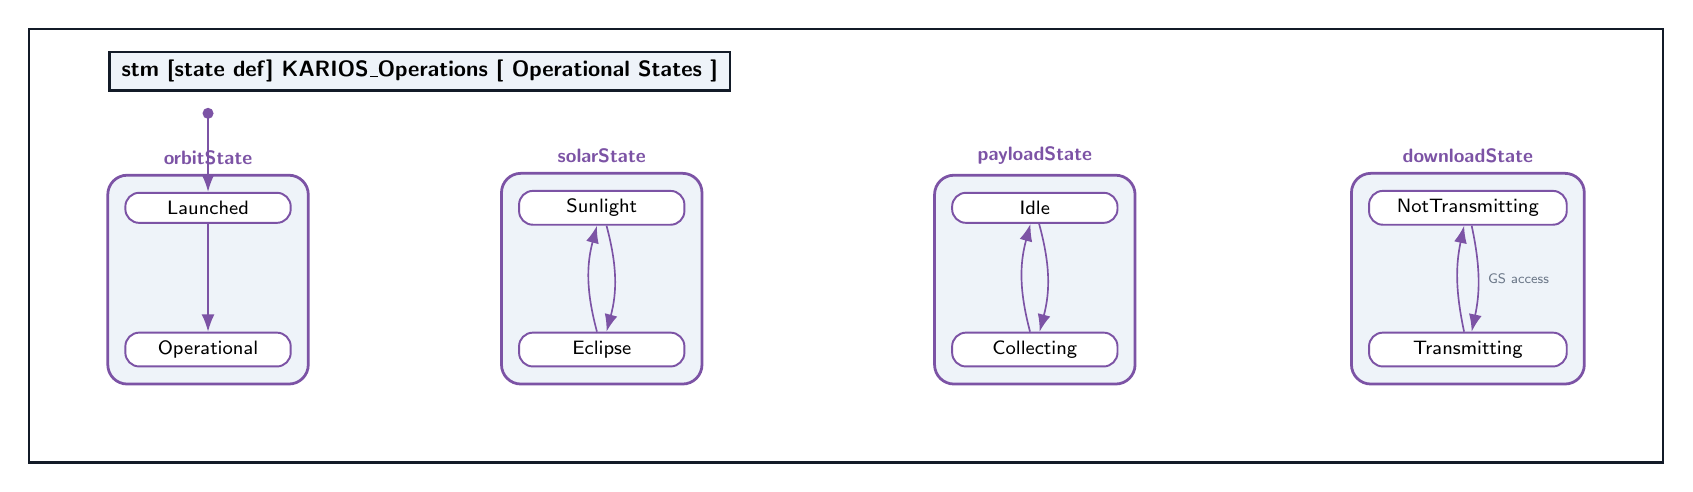
\begin{tikzpicture}[node distance=5mm]
\begin{scope}[local bounding box=bb]
  % Orbit region
  \node[st] (launched) at (-10,1.2) {Launched};
  \node[st] (operational) at (-10,-0.6) {Operational};
  \fill[cbeh] (-10,2.4) circle (2pt); \draw[tr] (-10,2.4) -- (launched);
  \draw[tr] (launched) -- (operational);
  % Solar region
  \node[st] (sun) at (-5,1.2) {Sunlight};
  \node[st] (ecl) at (-5,-0.6) {Eclipse};
  \draw[tr] (sun) to[bend left=15] (ecl); \draw[tr] (ecl) to[bend left=15] (sun);
  % Payload region
  \node[st] (idle) at (0.5,1.2) {Idle};
  \node[st] (coll) at (0.5,-0.6) {Collecting};
  \draw[tr] (idle) to[bend left=15] (coll); \draw[tr] (coll) to[bend left=15] (idle);
  % Download region
  \node[st, text width=2.3cm] (ntx) at (6,1.2) {NotTransmitting};
  \node[st, text width=2.3cm] (tx) at (6,-0.6) {Transmitting};
  \draw[tr] (ntx) to[bend left=12] node[midway,right,font=\tiny,text=ink3]{GS access} (tx);
  \draw[tr] (tx) to[bend left=12] (ntx);
  % composite-state boxes on the background so they don't cover substates
  \begin{scope}[on background layer]
    \node[cst, fit=(launched)(operational), label={[font=\scriptsize\bfseries,text=cbeh]above:orbitState}] (orb) {};
    \node[cst, fit=(sun)(ecl), label={[font=\scriptsize\bfseries,text=cbeh]above:solarState}] (sol) {};
    \node[cst, fit=(idle)(coll), label={[font=\scriptsize\bfseries,text=cbeh]above:payloadState}] (pl) {};
    \node[cst, fit=(ntx)(tx), label={[font=\scriptsize\bfseries,text=cbeh]above:downloadState}] (dl) {};
  \end{scope}
\end{scope}
\begin{scope}[on background layer]\node[frame, fit=(bb)]{};\end{scope}
\dtitle{stm [state def] KARIOS\_Operations [ Operational States ]}
\end{tikzpicture}

\clearpage
% =====================================================================
%  5.  PAR  --  PARAMETRIC (budgets as constraint blocks)
% =====================================================================
\begin{center}\small\textbf{Figure 5 --- Parametric Diagram (engineering budgets)}\end{center}
\begin{tikzpicture}
\begin{scope}[local bounding box=bb]
  % constraint blocks
  \node[cons] (pb) at (-8,1.5)
     {{\ster «constraint» PowerBudget}\\[2pt] $P_{array}(1-f_{ecl}) \geq P_{load}$};
  \node[cons] (db) at (0,1.5)
     {{\ster «constraint» DataBudget}\\[2pt] $R_{dl}\,t_{contact} \geq R_{col}\,t_{col}$};
  \node[cons] (lb) at (8,1.5)
     {{\ster «constraint» LinkBudget}\\[2pt] $EIRP - L_{path} + G/T \geq (E_b/N_0)_{req}$};
  \node[cons] (cb) at (-4,-3)
     {{\ster «constraint» CoverageBudget}\\[2pt] $t_{revisit} \leq t_{revisit,req}$};
  % value properties feeding them
  \node[vprop] (arr) at (-11,-1) {eps.arrayPower};
  \node[vprop] (load) at (-8.5,-1) {avgLoad};
  \node[vprop] (fecl) at (-6,-1) {orbit.eclipseFrac};
  \node[vprop] (rdl) at (-2,-1) {comm.loraRate};
  \node[vprop] (tc) at (0.2,-1) {STK: contactTime};
  \node[vprop] (rcol) at (2.4,-1) {sigint.rate};
  \node[vprop] (trev) at (-4,-5) {STK: revisitTime};
  % bindings
  \foreach \a in {arr,load,fecl}{ \draw[bind] (\a.north) -- (pb.south); }
  \foreach \a in {rdl,tc,rcol}{ \draw[bind] (\a.north) -- (db.south); }
  \draw[bind] (trev.north) -- (cb.south);
  % note linking to STK analysis
  \node[font=\scriptsize\itshape, text=ink3, text width=6cm, align=center] at (7,-3.2)
     {Constraint parameters bound to STK / MATLAB\\ results via ModelCenter (executable co-simulation).};
\end{scope}
\begin{scope}[on background layer]\node[frame, fit=(bb)]{};\end{scope}
\dtitle{par [package] Analysis [ KARIOS Engineering Budgets ]}
\end{tikzpicture}

\clearpage
% =====================================================================
%  6.  IBD  --  INTERNAL BLOCK DIAGRAM (spacecraft internal connections)
% =====================================================================
\begin{center}\small\textbf{Figure 6 --- Internal Block Diagram (Structure connections)}\end{center}
\begin{tikzpicture}
\begin{scope}[local bounding box=bb]
  % parts
  \node[ibdblk] (eps)  at (-7,1)   {\textbf{eps}\\[1pt]{\ster : EPS}};
  \node[ibdblk] (obc)  at (-2,1)   {\textbf{obc}\\[1pt]{\ster : OBC}};
  \node[ibdblk] (comm) at (3.5,1)  {\textbf{comm}\\[1pt]{\ster : Comms}};
  \node[ibdblk] (adcs) at (-2,4)   {\textbf{adcs}\\[1pt]{\ster : ADCS}};
  \node[ibdblk] (sig)  at (-5.5,-2.8) {\textbf{sigintPayload}};
  \node[ibdblk] (cyb)  at (1,-2.8)    {\textbf{cyberPayload}};
  % external spacecraft RF ports (on the frame, right side)
  \node[port,label={[font=\tiny]right:uhf}]  (uhf)  at (8,1.4) {};
  \node[port,label={[font=\tiny]right:lora}] (lora) at (8,0.4) {};
  % ---- ports (small squares) ----
  \node[port] (eps_o)  at (eps.east) {};
  \node[port] (eps_s)  at (eps.south) {};
  \node[port] (eps_n)  at (eps.north) {};
  \node[port] (obc_w)  at (obc.west) {};
  \node[port] (obc_e)  at (obc.east) {};
  \node[port] (obc_n)  at (obc.north) {};
  \node[port] (obc_sl) at ([xshift=-6mm]obc.south) {};
  \node[port] (obc_sr) at ([xshift=6mm]obc.south) {};
  \node[port] (adcs_s) at (adcs.south) {};
  \node[port] (adcs_w) at (adcs.west) {};
  \node[port] (comm_w) at (comm.west) {};
  \node[port] (comm_e1) at ([yshift=3mm]comm.east) {};
  \node[port] (comm_e2) at ([yshift=-3mm]comm.east) {};
  \node[port] (sig_e)  at (sig.east) {};
  \node[port] (cyb_n)  at (cyb.north) {};
  % ---- connections (orthogonal / straight) ----
  \draw[conn] (eps_o) -- (obc_w) node[midway,flowlbl]{«power»};                 % straight
  \draw[conn] (obc_e) -- (comm_w) node[midway,flowlbl]{«data»};                 % straight
  \draw[conn] (obc_n) -- (adcs_s) node[midway,flowlbl]{«cmd»};                  % straight
  \draw[conn] (eps_n) |- (adcs_w) node[pos=0.75,flowlbl]{«power»};              % up then across
  \draw[conn] (eps_s) -- ++(0,-1.1) -| (obc_sl);                               % power to obc (down/across/up)
  \draw[conn] (eps.south) -- ++(0,-1.6) -| (comm.south) node[pos=0.25,flowlbl]{«power»};
  \draw[conn] (sig_e) -| (obc_sl);                                             % data up into obc
  \draw[conn] (cyb_n) |- (obc_sr) node[pos=0.9,flowlbl]{«data»};               % data into obc
  \draw[conn] (comm_e1) -- (uhf) node[midway,flowlbl]{«RF»};                    % straight
  \draw[conn] (comm_e2) -- (lora);                                             % straight
\end{scope}
\begin{scope}[on background layer]\node[frame, fit=(bb)]{};\end{scope}
\dtitle{ibd [block] KARIOS\_Spacecraft [ Internal Connections ]}
\end{tikzpicture}

\clearpage
% =====================================================================
%  7.  ACT  --  ACTIVITY : Collect & Distribute Mission Data
% =====================================================================
\begin{center}\small\textbf{Figure 7 --- Activity Diagram: Collect \& Distribute Mission Data}\end{center}
\begin{tikzpicture}
\begin{scope}[local bounding box=bb]
  % ---- swimlanes (partitions) ----
  \foreach \x/\name in {-6/Payload, -2/OBC, 2/Comms, 6/{Ground Station}}{
     \node[font=\scriptsize\bfseries, text=ink] at (\x,3.4) {\name};
  }
  \foreach \x in {-4,0,4}{ \draw[line, densely dashed, draw=line, line width=0.6pt] (\x,3.1) -- (\x,-6); }
  % ---- nodes ----
  \fill[cbeh] (-2,2.7) circle (2.6pt);                                          % initial
  \node[act] (gen)   at (-2,1.6)  {Generate Mission Tasking};
  \node[act] (col)   at (-6,0.1)  {Collect Data};
  \node[act] (store) at (-2,-1.3) {Store On-Board};
  \node[dec] (dec)   at (-2,-3.0) {GS in view?};
  \node[act] (dl)    at (2,-4.2)  {Downlink Data};
  \node[act] (dist)  at (6,-4.2)  {Receive \& Distribute};
  \draw[cbeh, line width=0.8pt, fill=surface] (6,-5.7) circle (3.4pt);         % final ring
  \fill[cbeh] (6,-5.7) circle (1.8pt);
  % ---- control / object flows (orthogonal) ----
  \draw[aflow] (-2,2.7) -- (gen);                                              % straight
  \draw[aflow] (gen.west) -| (col.north) node[pos=0.75,flowlbl,text=cbeh]{tasking};
  \draw[aflow] (col.east) -| (store.north) node[pos=0.75,flowlbl,text=cstr]{«Raw Data»};
  \draw[aflow] (store) -- (dec);                                              % straight
  \draw[aflow] (dec.east) -| (dl.north) node[pos=0.2,guard]{[ in access ]};
  \draw[aflow] (dec.west) -- ++(-1.1,0) |- (store.west) node[pos=0.85,guard]{[ no access ]};
  \draw[aflow] (dl.east) -- (dist.west) node[midway,flowlbl,text=cstr]{«Data Frame»};  % straight
  \draw[aflow] (dist) -- (6,-5.36);                                           % straight to final
\end{scope}
\begin{scope}[on background layer]\node[frame, fit=(bb)]{};\end{scope}
\dtitle{act [activity] CollectAndDistributeMissionData}
\end{tikzpicture}

\end{document}
